
\documentclass[letterpaper,hide notes,xcolor={table,svgnames},pdftex,10pt]{beamer}
\def\showexamples{t}

\usecolortheme{crane}
\setbeamertemplate{navigation symbols}{}

\usetheme{MyPittsburgh}
\usepackage{hyperref}
\usepackage{graphicx,xspace}
\usepackage[normalem]{ulem}
\usepackage{multicol}
\usepackage{amsmath,amssymb,amsthm,graphicx,xspace}
\newcommand\SF[1]{$\bigstar$\footnote{SF: #1}}

\usepackage[sfdefault,lf]{carlito}
\usepackage[T1]{fontenc}
\usepackage[scaled]{beramono}
\usepackage{tikzpagenodes}
\newcommand{\Rplus}{\protect\hspace{-.1em}\protect\raisebox{.35ex}{\small{\small\textbf{+}}}}
\newcommand{\Cpp}{\mbox{C\Rplus\Rplus}\xspace}

\newcounter{tmpnumSlide}
\newcounter{tmpnumNote}

\newcommand\mnote[1]{%
	\addtocounter{tmpnumSlide}{1}
	\ifdefined\showcues {~\tiny\fbox{\arabic{tmpnumSlide}}}\fi
	\note{\setlength{\parskip}{1ex}\addtocounter{tmpnumNote}{1}\textbf{\Large \arabic{tmpnumNote}:} {#1\par}}}

\newcommand\mmnote[1]{\note{\setlength{\parskip}{1ex}#1\par}}


\newcommand\mquestion[2]{{~\color{red}\fbox{?}}\note{\setlength{\parskip}{1ex}\par{\Large \textbf{?}} #1} \note{\setlength{\parskip}{1ex}\par{\Large \textbf{A}} #2\par}\ifdefined \presentationonly \pause \fi}

\newcommand\blackboard[1]{%
	\ifdefined   \showblackboard
		{#1}
	\else {\begin{center} \fbox{\colorbox{blue!30}{%
						\begin{minipage}{.95\linewidth}%
							\hspace{\stretch{1}} Some space intentionally left blank; done at the blackboard.%
						\end{minipage}}}\end{center}}%
	\fi%
}

\usepackage{listings}
\lstset{%
	keywordstyle=\bfseries,
	aboveskip=15pt,
	belowskip=15pt,
	captionpos=b,
	identifierstyle=\ttfamily,
	frame=lines,
	numbers=left, basicstyle=\scriptsize, numberstyle=\tiny, stepnumber=0, numbersep=2pt}

\usepackage{siunitx}
\newcommand\sius[1]{\num[group-separator = {,}]{#1}\si{\micro\second}}
\newcommand\sims[1]{\num[group-separator = {,}]{#1}\si{\milli\second}}
\newcommand\sins[1]{\num[group-separator = {,}]{#1}\si{\nano\second}}
\sisetup{group-separator = {,}, group-digits = true}

%% -------------------- tikz --------------------
\usepackage{tikz}
\usetikzlibrary{positioning}
\usetikzlibrary{arrows,backgrounds,automata,decorations.shapes,decorations.pathmorphing,decorations.markings,decorations.text}

\tikzstyle{place}=[circle,draw=blue!50,fill=blue!20,thick, inner sep=0pt,minimum size=6mm]
\tikzstyle{transition}=[rectangle,draw=black!50,fill=black!20,thick, inner sep=0pt,minimum size=4mm]

\tikzstyle{block}=[rectangle,draw=black, thick, inner sep=5pt]
\tikzstyle{bullet}=[circle,draw=black, fill=black, thin, inner sep=2pt]

\tikzstyle{pre}=[<-,shorten <=1pt,>=stealth',semithick]
\tikzstyle{post}=[->,shorten >=1pt,>=stealth',semithick]
\tikzstyle{bi}=[<->,shorten >=1pt,shorten <=1pt, >=stealth',semithick]

\tikzstyle{mut}=[-,>=stealth',semithick]

\tikzstyle{treereset}=[dashed,->, shorten >=1pt,>=stealth',thin]

\usepackage{ifmtarg}
\usepackage{xifthen}
\makeatletter
% new counter to now which frame it is within the sequence
\newcounter{multiframecounter}
% initialize buffer for previously used frame title
\gdef\lastframetitle{\textit{undefined}}
% new environment for a multi-frame
\newenvironment{multiframe}[1][]{%
	\ifthenelse{\isempty{#1}}{%
		% if no frame title was set via optional parameter,
		% only increase sequence counter by 1
		\addtocounter{multiframecounter}{1}%
	}{%
		% new frame title has been provided, thus
		% reset sequence counter to 1 and buffer frame title for later use
		\setcounter{multiframecounter}{1}%
		\gdef\lastframetitle{#1}%
	}%
	% start conventional frame environment and
	% automatically set frame title followed by sequence counter
	\begin{frame}%
		\frametitle{\lastframetitle~{\normalfont(\arabic{multiframecounter})}}%
		}{%
	\end{frame}%
}
\makeatother

\makeatletter
\newdimen\tu@tmpa%
\newdimen\ydiffl%
\newdimen\xdiffl%
\newcommand\ydiff[2]{%
	\coordinate (tmpnamea) at (#1);%
	\coordinate (tmpnameb) at (#2);%
	\pgfextracty{\tu@tmpa}{\pgfpointanchor{tmpnamea}{center}}%
	\pgfextracty{\ydiffl}{\pgfpointanchor{tmpnameb}{center}}%
	\advance\ydiffl by -\tu@tmpa%
}
\newcommand\xdiff[2]{%
	\coordinate (tmpnamea) at (#1);%
	\coordinate (tmpnameb) at (#2);%
	\pgfextractx{\tu@tmpa}{\pgfpointanchor{tmpnamea}{center}}%
	\pgfextractx{\xdiffl}{\pgfpointanchor{tmpnameb}{center}}%
	\advance\xdiffl by -\tu@tmpa%
}
\makeatother
\newcommand{\copyrightbox}[3][r]{%
	\begin{tikzpicture}%
		\node[inner sep=0pt,minimum size=2em](ciimage){#2};
		\usefont{OT1}{phv}{n}{n}\fontsize{4}{4}\selectfont
		\ydiff{ciimage.south}{ciimage.north}
		\xdiff{ciimage.west}{ciimage.east}
		\ifthenelse{\equal{#1}{r}}{%
			\node[inner sep=0pt,right=1ex of ciimage.south east,anchor=north west,rotate=90]%
			{\raggedleft\color{black!50}\parbox{\the\ydiffl}{\raggedright{}#3}};%
		}{%
			\ifthenelse{\equal{#1}{l}}{%
				\node[inner sep=0pt,right=1ex of ciimage.south west,anchor=south west,rotate=90]%
				{\raggedleft\color{black!50}\parbox{\the\ydiffl}{\raggedright{}#3}};%
			}{%
				\node[inner sep=0pt,below=1ex of ciimage.south west,anchor=north west]%
				{\raggedleft\color{black!50}\parbox{\the\xdiffl}{\raggedright{}#3}};%
			}
		}
	\end{tikzpicture}
}


%% --------------------

%\usepackage[excludeor]{everyhook}
%\PushPreHook{par}{\setbox0=\lastbox\llap{MUH}}\box0}

%\vspace*{\stretch{1}

%\setbox0=\lastbox \llap{\textbullet\enskip}\box0}

\setlength{\parskip}{\fill}

\newcommand\noskips{\setlength{\parskip}{1ex}}
\newcommand\doskips{\setlength{\parskip}{\fill}}

\newcommand\xx{\par\vspace*{\stretch{1}}\par}
\newcommand\xxs{\par\vspace*{2ex}\par}
\newcommand\tuple[1]{\langle #1 \rangle}
\newcommand\code[1]{{\sf \footnotesize #1}}
\newcommand\ex[1]{\uline{Example:} \ifdefined \presentationonly \pause \fi
	\ifdefined\showexamples#1\xspace\else{\uline{\hspace*{2cm}}}\fi}

\newcommand\ceil[1]{\lceil #1 \rceil}


\AtBeginSection[]
{
	\begin{frame}
		\frametitle{Outline}
		\tableofcontents[currentsection]
	\end{frame}
}



\pgfdeclarelayer{edgelayer}
\pgfdeclarelayer{nodelayer}
\pgfsetlayers{edgelayer,nodelayer,main}

\tikzstyle{none}=[inner sep=0pt]
\tikzstyle{rn}=[circle,fill=Red,draw=Black,line width=0.8 pt]
\tikzstyle{gn}=[circle,fill=Lime,draw=Black,line width=0.8 pt]
\tikzstyle{yn}=[circle,fill=Yellow,draw=Black,line width=0.8 pt]
\tikzstyle{empty}=[circle,fill=White,draw=Black]
\tikzstyle{bw} = [rectangle, draw, fill=blue!20,
text width=4em, text centered, rounded corners, minimum height=2em]

\newcommand{\CcNote}[1]{% longname
	This work is licensed under the \textit{Creative Commons #1 3.0 License}.%
}
\newcommand{\CcImageBy}[1]{%
	\includegraphics[scale=#1]{creative_commons/cc_by_30.pdf}%
}
\newcommand{\CcImageSa}[1]{%
	\includegraphics[scale=#1]{creative_commons/cc_sa_30.pdf}%
}
\newcommand{\CcImageNc}[1]{%
	\includegraphics[scale=#1]{creative_commons/cc_nc_30.pdf}%
}
\newcommand{\CcGroupBySa}[2]{% zoom, gap
	\CcImageBy{#1}\hspace*{#2}\CcImageNc{#1}\hspace*{#2}\CcImageSa{#1}%
}
\newcommand{\CcLongnameByNcSa}{Attribution-NonCommercial-ShareAlike}

\newenvironment{changemargin}[1]{% 
	\begin{list}{}{% 
		\setlength{\topsep}{0pt}% 
		\setlength{\leftmargin}{#1}% 
		\setlength{\rightmargin}{1em}
		\setlength{\listparindent}{\parindent}% 
		\setlength{\itemindent}{\parindent}% 
		      \setlength{\parsep}{\parskip}% 
		      }% 
		\item[]}{\end{list}}




\title{Lecture 5 --- Interrupt Implementation }

\author{Jeff Zarnett \& Mike Cooper-Stachowsky \\ \small \texttt{jzarnett@uwaterloo.ca, mstachowsky@uwaterloo.ca}}
\institute{Department of Electrical and Computer Engineering \\
  University of Waterloo}
\date{\today}



\begin{document}

\begin{frame}
  \titlepage
  
  \small{Credit: Based on material from Allyson Giannikouris}

 \end{frame}

\begin{frame}
\frametitle{More About Interrupts}

The previous topic discussed interrupts, both hardware and software.

We also learned about how to deal with them on the Cortex M4.

But to truly understand them, we need to look deeper into hardware.

\end{frame}

\begin{frame}
\frametitle{Key Idea: No Polling}

Avoid polling as much as possible: it's a waste of time!

Instead: CPU can do whatever else is ready...\\
\quad And get alerted when something happens. 

\begin{center}
	
\includegraphics[width=0.4\textwidth]{images/alarmclock.jpg}
\end{center}

\end{frame}

\begin{frame}
\frametitle{Sleeping}

\begin{center}
	
\includegraphics[width=0.5\textwidth]{images/awakebeauty.jpg}
\end{center}

The CPU can be in a ``sleeping'' mode, but we're ignoring that for this course.

\end{frame}

\begin{frame}
\frametitle{Triggering an Interrupt}

What can cause an interrupt?

\begin{itemize}
	\item Clock signals
	\item Timers
	\item Peripherals (UART, SPI, I2C, GPIO, ADC...)
\end{itemize}

\end{frame}

\begin{frame}
\frametitle{Interrupt Time}

We covered 3 of the 4 items here last time:

\begin{enumerate}
	\item Interrupt the CPU
	\item Save the state of the current task (PC, SP, R0-R3, LR)
	\item Handle the interrupt
	\item Resume execution (unless it's hard fault or similar)
\end{enumerate}

But we didn't cover how the hardware interrupt works!


\end{frame}

\begin{frame}
\frametitle{How to get the CPU's Attention}

\begin{center}
	
\includegraphics[width=0.5\textwidth]{images/thor.jpg}
\end{center}

It's a physical voltage signal (the power of electricity!).

\end{frame}

\begin{frame}
\frametitle{How to get the CPU's Attention}

Each interrupt has a dedicated wire -- we call them \alert{line}s.

The line indicates the interrupt is ready.

The CPU has various interrupt registers to see if the interrupt is ready.

Signalling the processor is called an \alert{interrupt request (IRQ)}.

\end{frame}

\begin{frame}
\frametitle{IRQ Configuration}

Configuring the interrupts is a bit of a headache and at one time involved setting physical jumpers on cards to configure them.

\begin{center}
	
\includegraphics[width=0.4\textwidth]{images/oldmancloud.png}
\end{center}

But the idea is still a table of interrupts...

\end{frame}

\begin{frame}
\frametitle{Interrupt Vector Table}

We use an array of function pointers!

Each interrupt references a particular address in the array.

Cortex M's vector table starts at \texttt{0x0}.


\end{frame}

\begin{frame}
\frametitle{Interrupt Vector Table}

\begin{center}
	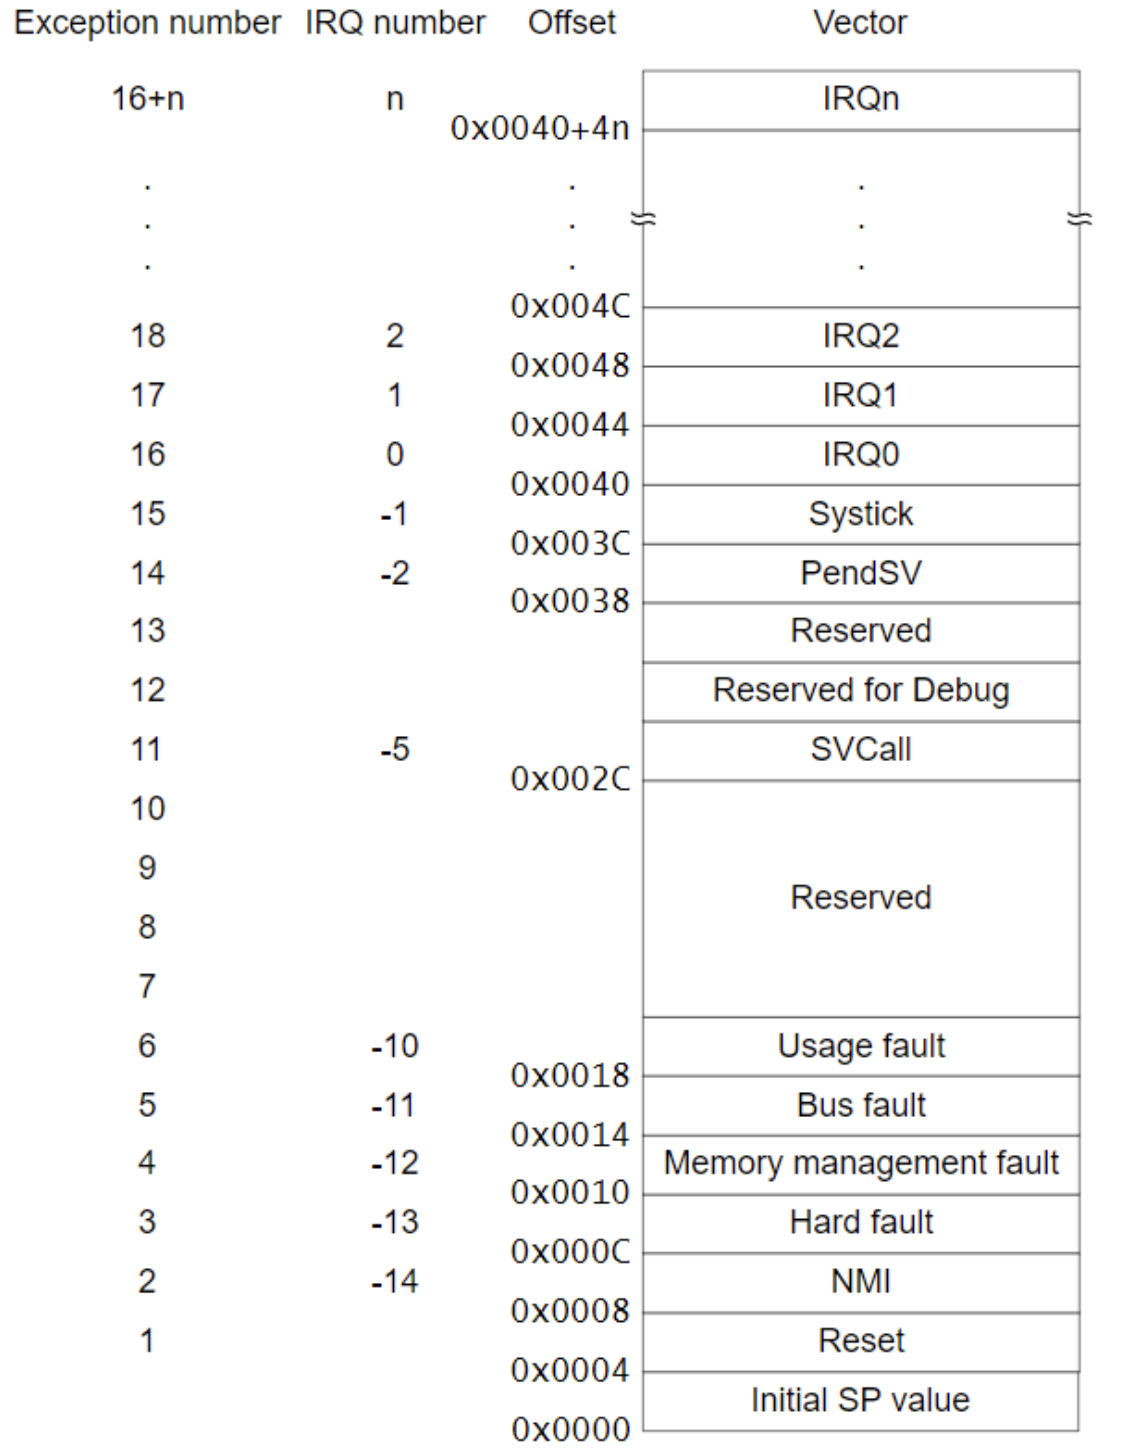
\includegraphics[width=0.5\textwidth]{images/ivt.png}
\end{center}

\end{frame}

\begin{frame}
\frametitle{That's a Relief}

Vector tables are configured in the setup code.

Good news: we almost never have to write it ourselves.

Pre-made code names the interrupt handler functions...\\
\quad And the names are used to write your IRQ functions.


\end{frame}

\begin{frame}
\frametitle{Example Config}

\begin{center}
	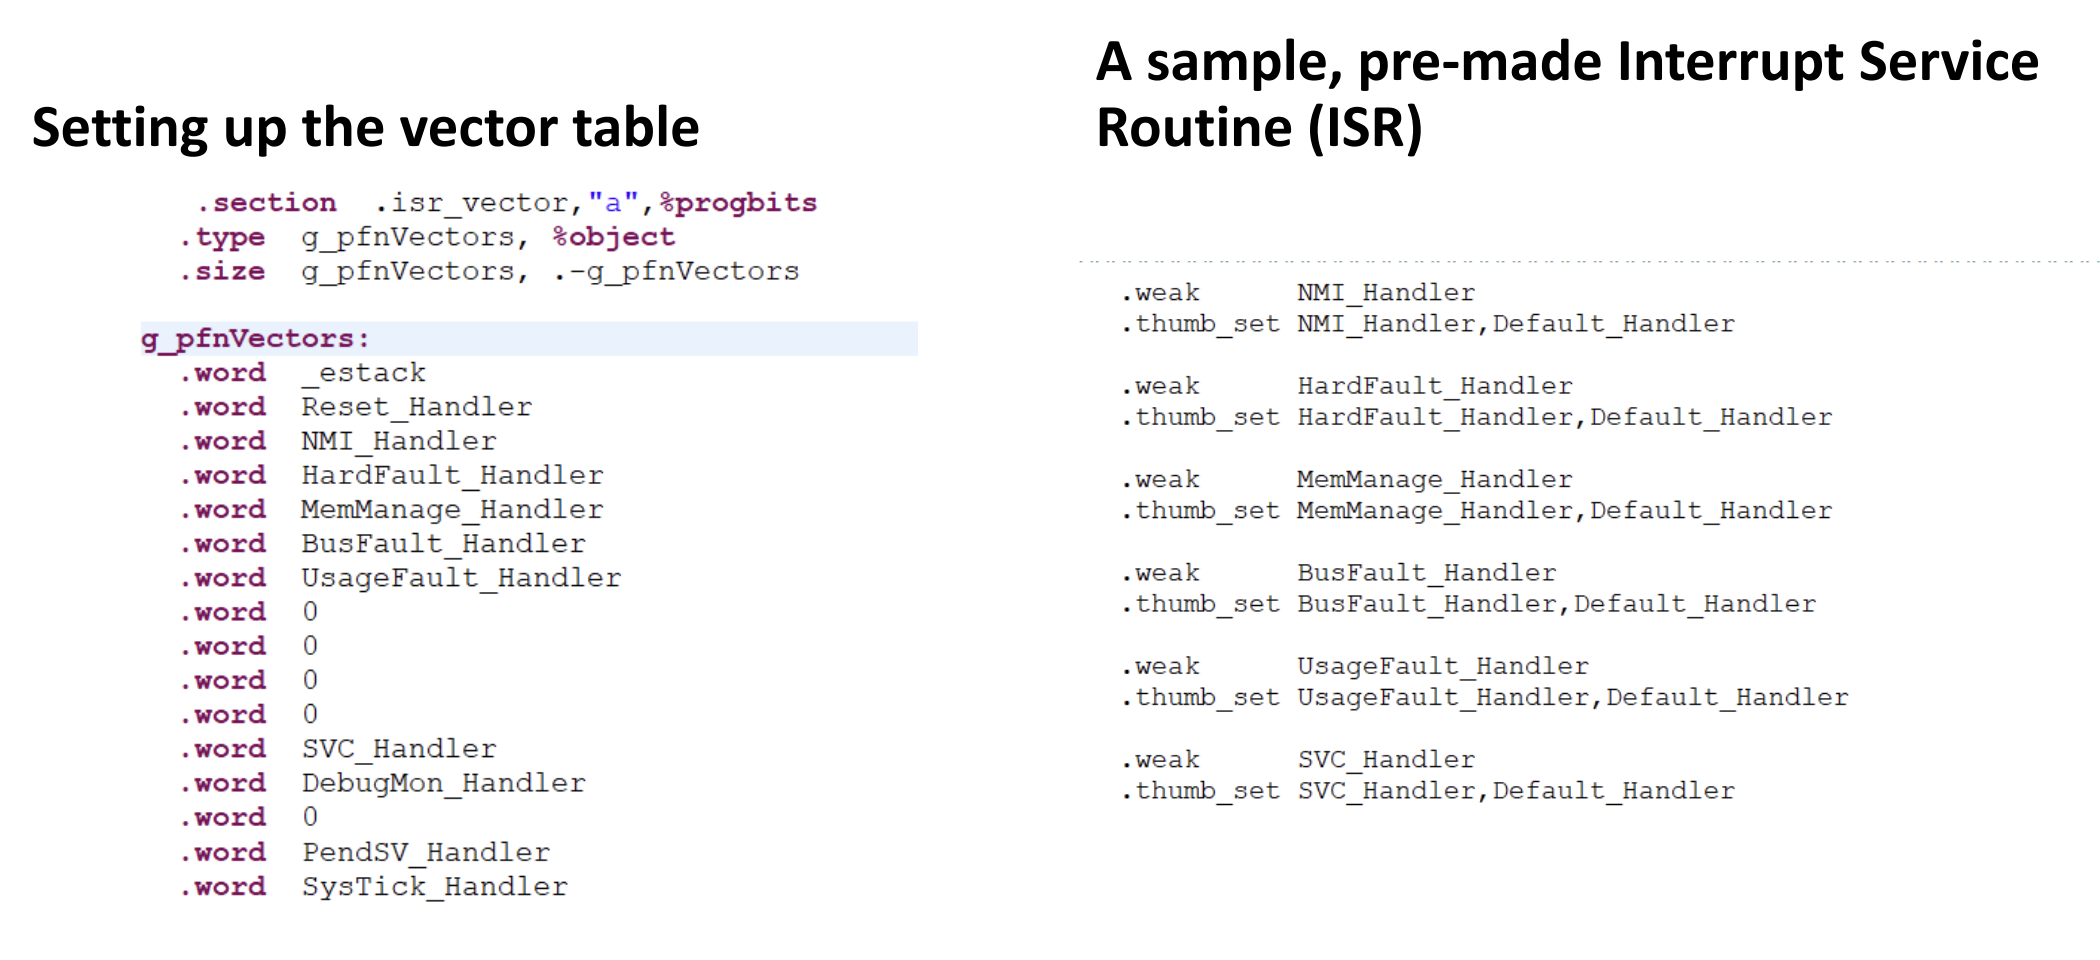
\includegraphics[width=\textwidth]{images/example-irq-config.png}
\end{center}


\end{frame}

\begin{frame}
\frametitle{Once Activated}

\begin{center}
	
\includegraphics[width=0.6\textwidth]{images/choppa.jpg}
\end{center}

This doesn't apply to SVC, though. 

\end{frame}

\begin{frame}[fragile]
\frametitle{Once Activated}

The code below runs when the SysTick interrupt happens, only if enabled.

\begin{lstlisting}[language=C]
void SysTick_Handler() {
  // Do the thing
}
\end{lstlisting}

Is it magical auto-generated design? Sure is.

\end{frame}

\begin{frame}
\frametitle{Gotta Go Fast}

Four main reasons to keep \alert{Interrupt Subroutines (ISRs)} short:

\begin{enumerate}
	\item Want to return to normal operation quickly
	\item Minimize the chance of other interrupts
	\item Shorter functions = less code = less risk of bug
	\item C is hard enough; Assembly is much harder
\end{enumerate}

\end{frame}

\begin{frame}
\frametitle{So Call Me Maybe?}

It's better to avoid calling functions in ISRs.

We'll learn more about why this is complex in a future topic. 

Functions called must be \alert{reentrant}. 

\end{frame}

\begin{frame}[fragile]
\frametitle{Non-Reentrant Code}

Any function that accesses a global or static variable is non-reentrant.

\begin{lstlisting}[language=C]
int tmp;
void swap( int *x, int *y ) {
  tmp = *x;
  *x = *y;
  *y = tmp; 
}
\end{lstlisting}

How would you fix this to make it reentrant? 

\end{frame}

\begin{frame}
\frametitle{All Done}

To return from an interrupt there's a special instruction \texttt{rti}.\\
\quad You cannot just do a regular \texttt{return} statement.

Let's think for a minute -- why not?

Usually the IDE helps you out here.

\end{frame}

\begin{frame}
\frametitle{Stop Talking While I'm Interrupting}

We know a few ways of handling interrupts during another interrupt:\\
\quad Ignore it, do it sequentially, switch to the new one?

But how to choose... by priority perhaps?

Interrupts are assigned a priority number; lower number is higher priority.\\
\quad At least in the Cortex M4; other systems are different.

\end{frame}

\begin{frame}
\frametitle{Stop Talking While I'm Interrupting}

Some interrupts are always at a high priority and we can't change that.\\
\quad Others are under our control!

We aren't going to handle nested interrupts in our OS (too hard).

\end{frame}

\begin{frame}
\frametitle{Maskable Interrupts}

Some interrupts are \alert{maskable}: can be ignored.

\begin{center}
	
\includegraphics[width=0.5\textwidth]{images/awesome.jpg}
\end{center}

IRQs fall in this category. Usually indicate non-critical things.

\end{frame}

\begin{frame}
\frametitle{Non-Maskable Interrupts}

Other interrupts are non-maskable (NMI).

\begin{center}
	
\includegraphics[width=0.5\textwidth]{images/prioritychannel.jpg}
\end{center}

Cannot be turned off or ignored; for critical things.

These force the CPU to halt execution!

\end{frame}

\begin{frame}
\frametitle{This is It}

In the Cortex M4 there's only one NMI.

It's the one that gets called when other interrupt handlers fault.

It's higher priority than anything other than \texttt{RESET}.

\end{frame}

\begin{frame}
\frametitle{Fault Priority Levels}

\begin{center}
	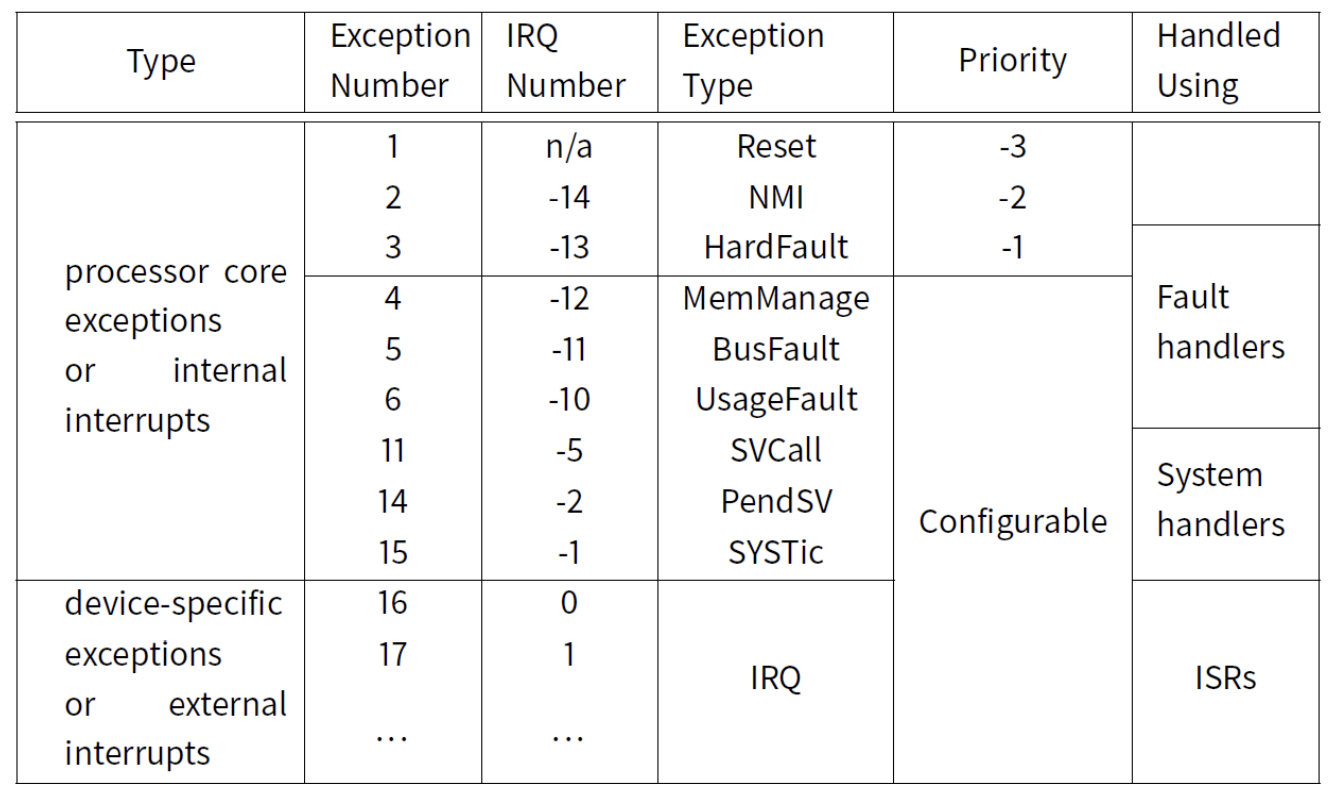
\includegraphics[width=0.95\textwidth]{images/fpl.png}
\end{center}

\end{frame}

\begin{frame}
\frametitle{IRQ States}

\textbf{Pending}: The conditions for the interrupt are met, but ISR has not run.

\textbf{Active}: The CPU is running the ISR.


\textbf{Pending and Active}: The next one is ready but we aren't done with the last!

\textbf{Inactive}: Neither pending nor active.


\end{frame}

\begin{frame}
\frametitle{Pending and Active}

Pending and active can happen if we're not keeping up with the speed of the device somehow, or the device isn't keeping up with the CPU.

\begin{center}
	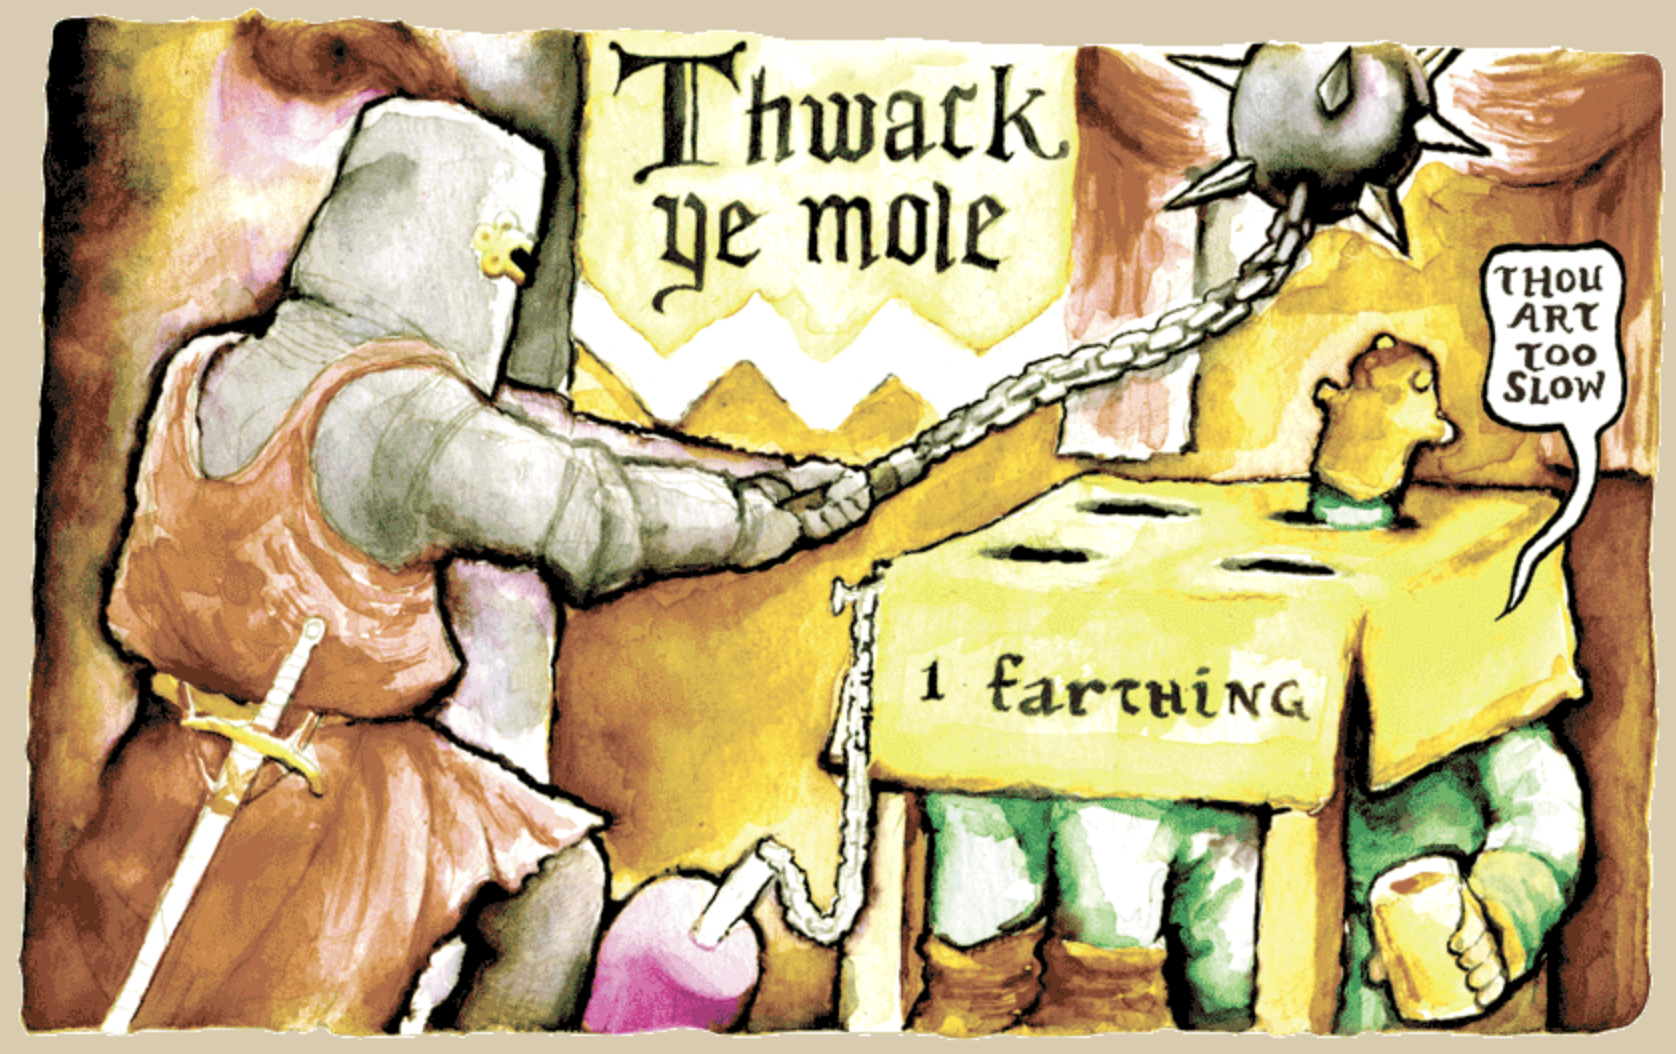
\includegraphics[width=0.5\textwidth]{images/tooslow.png}
\end{center}

Sometimes it's also about luck and timing; events can happen very close together.

\end{frame}

\begin{frame}
\frametitle{Global Interrupt Enable}

There is a single setting to turn on/off all interrupts.

When ``off'', if triggered, they go to the pending state.

When interrupts re-enabled, all pending ones evaluated by priority.

This does not turn off NMI.

\end{frame}

\begin{frame}
\frametitle{Is this Easy or Hard?}

When a hardware interrupt occurs, though, what does the ISR do?

Simple ISRs are easier to write but they can only do so much.

What if the interrupt handler just needs to tell a user program it can proceed?

\end{frame}

\begin{frame}
\frametitle{Don't forget to Like and Subscribe}

This takes us down an interesting path...

\begin{center}
	
\includegraphics[width=0.3\textwidth]{images/pandora.jpg}
\end{center}

Tasks (user processes) have state, more than just the current registers.

\end{frame}

\begin{frame}
\frametitle{Try Again Later}

We'll have to return to the subject of how tasks (processes and threads) can be made to wait when they're not able to continue.

Just to be clear, what we're talking about is context-switching and multi-threading, but we're not ready for that yet.

It will come up soon and will be important in the labs.

\end{frame}

\begin{frame}
\frametitle{On to Hardware Devices Then}

Before we're ready to go on, we need to spend some more time on hardware.

\begin{center}
	
\includegraphics[width=0.5\textwidth]{images/cable_hell.jpg}
\end{center}

Our next topic will focus on communicating with hardware devices!

\end{frame}

\end{document}

